\subsection{Automatic Verification of Security Properties}\label{SecVerif}

As explained above, we are interested in the verification of
high-level security properties that are not directly related to a
single method or class, but that guarantee the overall
well-functioning of an application. Writing appropriate JML
annotations for such properties is tedious and error-prone, as they
have to be spread all over the application. Therefore, we propose a
way to construct such annotations automatically. First we synthesise
core-annotations for methods directly involved in the property.  For
example, when specifying that no nested transactions are allowed, we
annotate the methods \texttt{beginTransaction},
\texttt{commitTransaction} and
\texttt{abortTransaction}. Subsequently, we propagate the necessary 
annotations to all methods (directly or indirectly) invoking these
core-methods.  The generated annotations are sufficient to respect the
security properties, \emph{i.e.}~if the applet does not violate the
annotations, it respects the corresponding high-level security
property.

Whether the applet respects its annotations can be established with
any of the existing tools for JML. We use JACK~\cite{BRL-JACK}, which
generates proof obligations for different provers, including the
AtelierB prover\footnote{\texttt{http://www.atelierb.societe.com/}}
and
Simplify\footnote{\texttt{http://research.compaq.com/SRC/esc/Simplify.html}}.
Both are automatic verifiers for first-order logical formulae. Since
for most security properties the annotations are relatively
simple---but there are many---it is important that these verifications
are done automatically, without any user interaction. The results in
Section~\ref{SecResults} show that for the generated annotations all
correct proof obligations can indeed be automatically discharged.

Before presenting the overall architecture of our tool set and
outlining the algorithm for propagation of annotations, we briefly
present a few JML keywords, that are relevant for the examples
presented here.

\subsubsection{JML in a Nutshell}\label{SubSecJML}

JML~\cite{BurdyCCEKLLP03} uses a Java-like syntax to write predicates,
extended with several specification-specific constructs, such as
\texttt{\bsl forall},
\texttt{\bsl exists} \emph{etc.} Method specifications consist of 
preconditions (\texttt{requires}), postconditions (\texttt{ensures}),
and exceptional postconditions (\texttt{exsures}), \emph{i.e.}\/~the
condition that has to hold upon abnormal termination of a method. We
can also specify so-called
\texttt{assignable} clauses, stating which variables may be modified
by a method. Class invariants (keyword \texttt{invariant}) describe
properties that have to be preserved by each method.

To write more abstract and implementation-independent specifications,
JML provides several means of abstraction. One of these are 
so-called ghost-variables, which are visible only in
specifications. Their declaration is preceded by the keyword
\texttt{ghost}. A special assignment annotation \texttt{set} allows
to update their value. Using invariants they can be related to concrete
variables.

A large class of security properties can be expressed using static
ghost variables of primitive type; these are typically used to keep
track of the control state of the application (including the ones
presented in Section~\ref{SecHighLevelSecProp}). Therefore, here we
only study the propagation of annotations containing static ghost
variables of primitive type. However, our propagation technique easily
can be generalised to concrete (static) variables, as long as we do
not have to handle aliasing.


%only . The reason for which only ghost variables are considered is that adding a java field for specification purposes means also modification in the code which can be avoided with ghost variables (not visible for a java compiler). Since in this paper we
%restrict our attention to these properties,  The static ghost variables are 
 

To give an example JML specification, we show a fragment of the
core-annotation for the \textbf{No nested transactions} property.  A
static ghost variable \texttt{TRANS} is declared that keeps track
of whether there is a transaction in progress. It is initialised to 0,
denoting that there is no transaction in progress.
\begin{verbatim}
/*@ static ghost int TRANS == 0; @*/
\end{verbatim}
The method \texttt{beginTransaction} is annotated as follows.
\begin{verbatim}
/*@ requires TRANS == 0;
  @ assignable TRANS;
  @ ensures TRANS == 1; @*/
public static native void beginTransaction() 
                          throws TransactionException;
\end{verbatim}
Since the method is native, one cannot describe its body. However, if
it had been non-native, an annotation \texttt{//@ set TRANS = 1;}
would have been generated, to ensure that the method satisfies its
specification.

\subsubsection{Architecture}

\begin{figure}[p]
\begin{center}
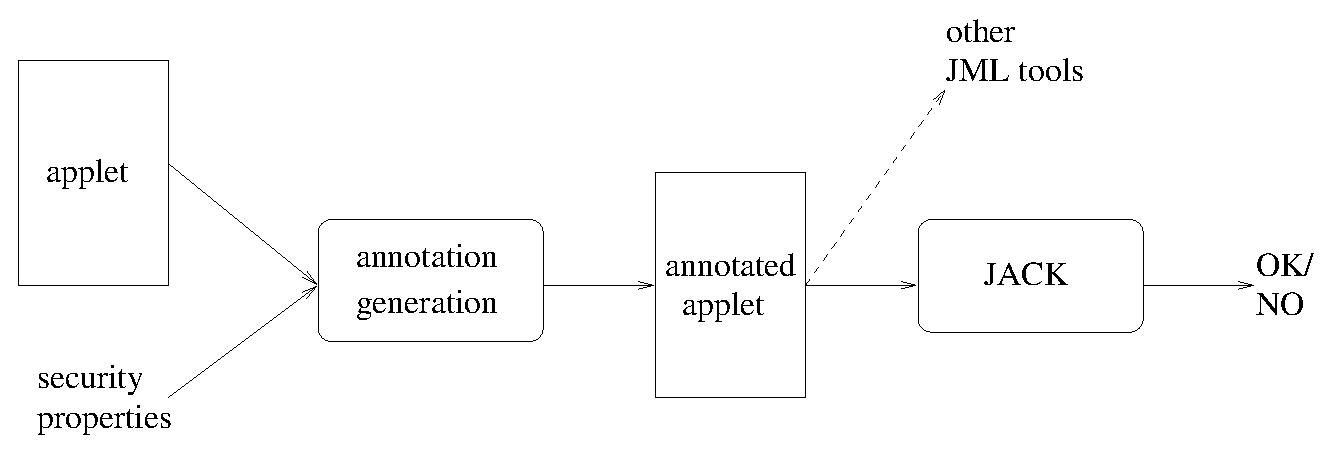
\epsfig{file=isaac/architecture.eps, width=9cm}
\end{center}
\caption{Tool set for verifying high-level security properties}\label{FigArch}
\end{figure}



Figure~\ref{FigArch} shows the general architecture of the tool set
for verifying high-level security properties. Our annotation generator
can be used as a front-end for any tool accepting JML-annotated Java
(Card) applications. As input we have a security property and a Java
Card applet. The output is a JML Abstract Syntax Tree (AST), using the
format as defined for the standard JML parser. When pretty-printed,
this AST corresponds to a JML-annotated Java file. From this
annotated file, JACK generates appropriate proof obligations to check
whether the applet respects the security property.

\subsubsection{Automatic Generation of Annotations}

Section~\ref{SecResults} presents example core-annotations for some of
the security properties presented in
Section~\ref{SecHighLevelSecProp}, here we focus on the weaving phase,
\emph{i.e.}~how the core-annotations are propagated throughout the
applet. We define functions \textsf{mod}, \textsf{pre}, \textsf{post} and
\textsf{exc\-post}, propagating assignable clauses, preconditions, 
postconditions and exceptional postconditions, respectively. These
functions have been defined and implemented for the full Java Card
language, but to present our ideas, we only give the definitions for a
representative subset of statements: statement composition, method
calls, conditional and \texttt{try}-\texttt{catch} statements and
special set-annotations. We assume the existence of domains
\textsf{MethName} of method names, \textsf{Stmt} of Java Card
statements, \textsf{Expr} of Java Card expressions, and \textsf{Var}
of static ghost variables, and functions
\textsf{call} and \textsf{body}, denoting a method call and 
body, respectively.

All functions are defined as mutual recursive functions on method
names, statements and expressions. When a method call is encountered,
the implementation will check whether annotations already have been
generated for this method (either by synthesising or weaving). If not
it will recursively generate appropriate annotations. Java Card
applets typically do not contain (mutually) recursive method calls,
therefore this does not cause any problems. Generating appropriate
annotations for recursive methods would require more care (and in
general it might not be possible to do without any user interaction).

\paragraph{Propagation of assignable clauses}
First we define a function \textsf{mod} that propagates
assignable clauses for static ghost variables.

%Different from the standard JML set of modified variables in a method, that takes into account  both JML and 
%Java variables, we keep track only of JML ghost static variables. For our purposes this is sufficient because the generated pre- and postconditions involve only ghost variables.
\begin{definition}[\textsf{mod}]We define functions
%\[
%\begin{array}{rcl}
\(\mathsf{mod} \colon \mathsf{MethName} \rightarrow
\mathcal{P}(\mathsf{Var})\), 
\(
\mathsf{mod}  \colon  \mathsf{Stmt}   \rightarrow
\mathcal{P}(\mathsf{Var}) \), and 
\(\mathsf{mod}  \colon  \mathsf{Expr}   \rightarrow  \mathcal{P}(\mathsf{Var})\)
%\end{array}
%\]
by rules like (where \(m,n\,\colon\mathsf{MethName}\),
\(s_1,s_2\,\colon\mathsf{Stmt}\), \(c\,\colon\mathsf{Expr}\) and \(x\colon\mathsf{Var}\)):
\[
\begin{array}{rcl}
\mathsf{mod}(m) & = & \mathsf{mod}(\mathsf{body}(m)) \smallskip \\
\mathsf{mod}(s_1 \mathtt{;} s_2) & = & \mathsf{mod}(s_1) \cup \mathsf{mod}(s_2)\\
\mathsf{mod}(\mathsf{call}(n)) & = &  \mathsf{mod}(n) \\
\mathsf{mod}(\mathtt{if\:(} c \mathtt{)\:} s_1 \mathtt{\:else\:} s_2)
&=& \mathsf{mod}(c) \cup \mathsf{mod}(s_1) \cup \mathsf{mod}(s_2)\\
\mathsf{mod}(\mathtt{try\:} s_1 \mathtt{\:catch\:(} E \mathtt{)\:}
s_2) & = & \mathsf{mod}(s_1) \cup \mathsf{mod}(s_2)\\
\mathsf{mod}(\mathtt{set\:}x \mathtt{\:=\:} c) & = &  \{ x \} 
\end{array}
\]
\end{definition}


\paragraph{Propagation of preconditions}
Next, we define a function \textsf{pre} for
propagating preconditions. This function analyses a
method body in a sequential way---from beginning to end---computing
which preconditions of the methods called within the body have to be
propagated. To understand the reasoning behind the definition, we will
first look at an example. Suppose we are checking the \textbf{No
nested transactions} property for an application, which contains a
method \texttt{m}, whose only method calls are those shown, and which
does not contain any set annotations.
\begin{verbatim}
void m() { ... // some internal computations
           JCSystem.beginTransaction();
           ... // computations within transaction
           JCSystem.commitTransaction(); }
\end{verbatim}
Core-annotations are synthesised for \texttt{beginTransaction}
and \texttt{commit\-Transaction}. The annotations for
\texttt{beginTransaction} are shown in Section~\ref{SubSecJML}
above, while \texttt{commitTransaction} requires \texttt{TRANS == 1}
and ensures \texttt{TRANS == 0}. As we assume that \texttt{TRANS} is
not modified by the code that precedes the call to
\texttt{beginTransaction},  the only way the precondition of this method
can hold, is by requiring that it already holds at the moment
\texttt{m} is called. Thus, the precondition of
\texttt{beginTransaction} has to be propagated. In contrast, the
precondition for \texttt{commitTransaction} (\texttt{TRANS == 1})
has to be established by the postcondition of
\texttt{begin\-Transaction}, because the variable \texttt{TRANS} is
modified by this method. %Propagating the precondition of
%\texttt{commit\-Transaction} to the precondition of \texttt{m} would
%not help to guarantee that the precondition of
%\texttt{commitTransaction} holds. 
Thus, preconditions containing only unmodified variables should be
propagated.  Propagating pre- or postconditions can be considered as
passing on a method contract. Method bodies can only pass on contracts
for variables they do not modify; once they modify a variable it is
their duty to ensure that the necessary conditions are satisfied.

%In the definition of the function \textsf{pre} for propagating
%preconditions, we assume the existence of a function \textsf{mod}
%returning the set of static ghost variables modified by a
%statement. 
%As we are only interested in static ghost variables with
%primitive types, the definition is straightforward and it does not
%have to consider aliasing. 

We assume the existence of a domain \textsf{Pred} of predicates using
static ghost variables only, and function
\textsf{fv}, returning the set of free variables.

%We define \textsf{pre} on method names, statements and
%expressions. These definitions are mutually recursive.  Java Card
%applets typically do not contain (mutually) recursive method calls,
%therefore this does not cause any problems. Generating appropriate
%annotations for recursive methods would require more care (and in
%general it might not be possible to do without any user interaction).
%\begin{definition} [\textsf{pre\_init}]
%\[
%\begin{array}{rcl}
%\mathsf{pre\_init}& \colon & \mathsf{MethName} \rightarrow  \mathcal{P}(\mathsf{Pred})
%\end{array}
%\]
%\end{definition}
%The function $\textsf{pre\_init}$ returns the predicate that a method declaration is initialised with. Such an initialisation can be seen 
%for example as the specification added for the  ``core'' methods. It is in fact any pre- or postcondition specified for a method before applying the functions that  we define.  
\begin{definition}[\textsf{pre}]
We define
%\[
%\begin{array}{rcl}
\(\mathsf{pre} \colon \mathsf{MethName} \rightarrow
\mathcal{P}(\mathsf{Pred})\),
\( \mathsf{pre}  \colon  \mathsf{Stmt} \rightarrow
\mathcal{P}(\mathsf{Var}) \rightarrow \mathcal{P}(\mathsf{Pred}) \), and
\( \mathsf{pre}  \colon  \mathsf{Expr} \rightarrow
\mathcal{P}(\mathsf{Var}) \rightarrow \mathcal{P}(\mathsf{Pred}) \)
%\end{array}
%\]
by rules like (where \(m,n\,\colon\mathsf{MethName}\),
\(s_1,s_2\,\colon\mathsf{Stmt}\), \(c\,\colon\mathsf{Expr}\),
\(V\colon\mathcal{P}(\mathsf{Var})\) and \(x\colon\mathsf{Var}\)): 
\[
\begin{array}{rcl}
\mathsf{pre}(m) & = & \mathsf{pre}(\mathsf{body}(m), \emptyset) \smallskip\\
\mathsf{pre}(s_1 \mathtt{;} s_2, V) & = & \mathsf{pre}(s_1, V) \cup 
                                          \mathsf{pre}(s_2, V \cup \mathsf{mod}(s_1))\\

\mathsf{pre}(\mathsf{call}(n),V) & = & 
                \{ p \mid p \in \mathsf{pre}(n) \wedge 
                          (\mathsf{fv}(p) \cap V) = \emptyset\}\\
\mathsf{pre}(\mathtt{if\:(} c \mathtt{)\:} s_1 \mathtt{\:else\:} s_2, V) & = &
   \mathsf{pre}(c, V) \cup 
   \mathsf{pre}(s_1, V \cup \mathsf{mod}(c)) \cup\\
&&   \mathsf{pre}(s_2, V \cup \mathsf{mod}(c))\\
\mathsf{pre}(\mathtt{try\:} s_1 \mathtt{\:catch\:(} E \mathtt{)\:} s_2, V) & = & 
   \mathsf{pre}(s_1, V) \cup 
   \mathsf{pre}(s_2, V \cup \mathsf{mod}(s1))\\
\mathsf{pre}( \mathtt{set\:} x \mathtt{\:=\:} c) & = & \{\: \}
\end{array}
\]
\end{definition}

In the rules defining \textsf{pre} on \textsf{Stmt} and \textsf{Expr},
the second argument denotes the set of static ghost variables that have been
modified so far. When calculating the precondition for a method, we
calculate the precondition of its body, assuming that so far no variables
have been modified. For a statement composition, we first
propagate the preconditions for the first sub-statement, and then for
the second sub-statement, but taking into account the variables
modified by the first sub-statement. When propagating the preconditions
for a method call, we propagate all preconditions of the called method
that do not contain modified variables.  Since we are restricting our
annotations to expressions containing static ghost variables only, in
the rule for the conditional statement we cannot take the outcome of
the conditional expression into account. As a consequence, we
sometimes generate too strong annotations, but in practice this does
not cause problems. Moreover, it should be emphasised that this
only can make us reject correct applets, but it will never make us
accept incorrect ones.  Similarly, for the
\texttt{try}-\texttt{catch} statement, we always propagate the
precondition for the \texttt{catch} clause, without checking whether it
actually can get executed. Again, this will only make us reject
correct applets, but it will never make us accept incorrect
ones. Finally, a set annotation does not give rise to any propagated
precondition. 

Notice that by definition, we have the following property for the
function \textsf{pre} (where \(s\) is either in \textsf{Stmt} or
\textsf{Expr}, and \(V\) is a set of static ghost variables).
\[
p \in \textsf{pre}(s, V) \Leftrightarrow (p \in \textsf{pre}(s,
\emptyset) \wedge (\textsf{fv}(p) \cap V) = \emptyset)
\]

\paragraph{Propagation of postconditions}
In a similar way, we define functions \textsf{post} and
\textsf{exc\-post},  computing the
set of postconditions and exceptional postconditions that have to be
propagated for method names, statements and expressions. The main
difference with the definition of \textsf{pre} is that these functions run
through a method from the end to the beginning. Moreover, they have to
take into account the different paths through the method. For
each of these possible paths, we calculate the appropriate
(exceptional) postcondition. The overall (exceptional) postcondition
is then defined as the disjunction of the postconditions related to
the different paths through the method. 

\paragraph{Example}
For the example discussed above, our functions compute the following
annotations.

\begin{verbatim}
/*@ requires TRANS == 0;
  @ assignable TRANS;
  @ ensures TRANS == 0; @*/
void m() { 
   ... // some internal computations
  JCSystem.beginTransaction();
  ... // computations within transaction
  JCSystem.commitTransaction(); }
\end{verbatim}
This might seem trivial, but it is important to realise that similar
annotations will be generated for all methods calling
\texttt{m}, and transitively for all methods calling the methods
calling \texttt{m} \emph{etc.}
Having an algorithm to generate such annotations enables to check
automatically a large class of high-level security properties.

\subsubsection{Annotation Generation and Predicate Transformer Calculi}
A natural question that arises is whether there is a relation between
our propagation functions and well-known program transformation calculi as
the weakest precondition (\textsf{wp}) and strongest postcondition
(\textsf{sp}).

The conceptual difference between our propagation functions and
standard program transformation calculi is that, given method \(m\)
our functions extract a method contract for \(m\), while the program
transformation calculi compute the proof obligations that, given all
method contracts, allow to decide whether the implementation of \(m\)
is correct.

%What should be pointed out is that there is a conceptual difference between 
%what functions \textsf{pre} and \textsf{post} calculate and what respectively weakest precondition(\textsf{wp}) 
%and strongest postcondition(\textsf{sp}) do. Let us look at \textsf{pre} and 
%\textsf{wp}. Function \textsf{pre} extracts logical information for a method \textsf{m} that indicates
%what any other method that may call \textsf{m}, should establish, i.e. \textsf{pre} calculates 
%a contract between methods based on a given specification. On the other hand \textsf{wp} gives a predicate upon which proof 
%obligations will be generated, i.e.\textsf{wp} tells us what should be provable in order to be able to conclude that a method 
%respects that given specification.

A formal relation between \textsf{pre} and (a variant of) the
\textsf{wp}-calculus can be established. Since we only consider ghost
variables, we need to consider an abstract version of the \textsf{wp}:
\textsf{wp}\(^{\#}\), which does not consider concrete
variables. Most rules of this abstract \textsf{wp}-calculus are
unchanged, but rules as for the conditional statement cannot consider
the outcome of the conditional expression.
\[
\mathsf{wp}^{\#}(\mathtt{if (}c\mathtt{)}s_1\mathtt{\:else\:}s_2,Q) =
\mathsf{wp}^{\#}(c, \mathsf{wp}^{\#}(s_1, Q)) \wedge
\mathsf{wp}^{\#}(c, \mathsf{wp}^{\#}(s_2, Q))
\]

The abstract \textsf{wp}-calculus is sound, that is every program that
can be proven correct with the abstract \textsf{wp}-calculus, can also
be proven correct with the standard \textsf{wp}-calculus.

\begin{lemma} For any statement \(s\), and any predicates \(P\) and
\(Q\), containing static ghost variables only, we have:
\[
\forall P, Q\colon\mathsf{Pred}, s\colon\mathsf{Stmt}. 
(P \Rightarrow \mathsf{wp}^{\#}(s, Q)) \Rightarrow (P \Rightarrow
\mathsf{wp}(s, Q))
\]
\end{lemma}


Now we  can prove a correspondence between \textsf{pre} and
\textsf{wp}\(^{\#}\). 


\begin{theorem}[Correspondence]
For any statement \(s\), its abstract weakest precondition is
equivalent to the calculated precondition, in conjunction with a
universally quantified expression \(F\).
\[
\exists F\colon\mathsf{Pred}.  
             \mathsf{wp}^{\#}(s, \lambda x. \mathsf{true}) = 
             (\mathsf{pre}(s, \emptyset) \wedge \forall
              \mathsf{mod}(s). F) 
\]
\end{theorem}

This property formalises the conceptual difference described above:
the function \textsf{pre} extracts the ``external'' part of the
\textsf{wp}\(^{\#}\) (the method contract), while the quantified
expression \(F\) corresponds to the ``internal'' proof obligations.
The proofs of both properties proceed by structural induction.
We believe similar equivalences can be proven for the function
\textsf{post} and the \textsf{sp}-calculus. However, we
are not aware of any adaptation of the \textsf{sp}-calculus to Java,
therefore we did not study this.



%The second
%property tells us that function \textsf{pre} ``extracts'' the free
%part of the result of \textsf{wp}\(^{\#}\). This means that proving
%\textsf{pre} is part of establishing that method implementation is correct (when its specification contains static ghost variabls of basic type only).
